\documentclass{article}
\usepackage[utf8]{inputenc}
\usepackage{amsmath}
\usepackage{amsfonts}
\usepackage{graphicx}
\usepackage{geometry}
\usepackage{hyperref}
\geometry{letterpaper, margin=1in}

\begin{document}
% Horizontal line

\vspace{-1cm}
\hrule
% Centered title
\begin{center}
    \LARGE \textbf{EMCH 394} \\
    \Large Final Project \\
    \large William Charles Wenzel \& Tanner Reid Haralson
\end{center}

% Horizontal line
\hrule
\vspace{0.2cm}

\section{Calculation of Moisture Content (Humidity Ratio)}

To determine the moisture content, or humidity ratio, we evaluate relative humidity effects on vapor pressures at 35°C. The saturation vapor pressure ($e_s$) is:
\[ e_s = 5.628 \, \text{kPa} \]
At 90\% relative humidity, the actual vapor pressure ($e$) becomes:
\[ e = 5.628 \times 0.90 = 5.0652 \, \text{kPa} \]
The humidity ratio ($\omega$), the mass of water vapor per mass of dry air, is:
\[ \omega = 0.622 \frac{5.0652}{101.325 - 5.0652} \approx 0.03273 \]

\section{Calculation of Total Air Volume}

Essential for HVAC designs, the air volume flow rate conversion from cubic meters per hour to seconds is:
\[ \dot{V}_{\text{air total}} = 3100 \, \text{m}^3/\text{hr} \]
Using 3600 seconds per hour for conversion:
\[ \dot{V}_{\text{air total}} \text{ in m}^3/\text{s} = \frac{3100}{3600} \approx 0.861 \, \text{m}^3/\text{s} \]

\section{Calculation of Moist Air Volume}
The volume of moist air (\( \dot{V}_{\text{moist air}} \)) is calculated using the total air volume and the humidity ratio:
\[ \dot{V}_{\text{moist air}} = \omega \times \dot{V}_{\text{air total}} \]
\noindent
First, convert the total air volume from cubic meters per hour to cubic meters per second:
\[ \dot{V}_{\text{air total}} \text{ in m}^3/\text{s} = \frac{3100 \, \text{m}^3/\text{hr}}{3600 \, \text{s/hr}} \approx 0.861 \, \text{m}^3/\text{s} \]
\noindent
Then, calculate the moist air volume:
\[ \dot{V}_{\text{moist air}} = 0.03273 \times 0.861 \, \text{m}^3/\text{s} \approx 0.02818 \, \text{m}^3/\text{s} \]
\noindent
The calculated moist air volume is approximately 0.02818 m³/s or \( 0.02818 \times 3600 \, \text{m}^3/\text{hr} \approx 101.45 \, \text{m}^3/\text{hr} \).

\section{Calculation of Dry Air Volume}
\noindent
The volume of dry air (\( \dot{V}_{\text{dry air}} \)) is the total air volume minus the volume of moist air:
\[ \dot{V}_{\text{dry air}} = \dot{V}_{\text{air total}} - \dot{V}_{\text{moist air}} \]
\noindent
Using the given total air volume and the calculated moist air volume, calculate the dry air volume:

\[ \dot{V}_{\text{dry air}} \text{ in m}^3/\text{s} = \frac{3100 \, \text{m}^3/\text{hr} - 101.45 \, \text{m}^3/\text{hr}}{3600 \, \text{s/hr}} \approx 0.83293 \, \text{m}^3/\text{s} \]
\noindent
The calculated dry air volume is approximately 0.83293 m³/s or \( 0.83293 \times 3600 \, \text{m}^3/\text{hr} \approx 2998.55 \, \text{m}^3/\text{hr} \).

\section{Calculation of Mass Flow Rate of Dry Air}

\begin{itemize}
    \item \( \dot{V}_{\text{dry air}} \approx 2998.55 \, \text{m}^3/\text{hr} \) (previously calculated)
    \item \( T_{\text{outside}} = 35^\circ\text{C} \) (approx.  \( 308.15 \, \text{K} \))
    \item \( P = 101.325 \, \text{kPa} \)
    \item \( R = 0.287 \, \text{kJ/kg} \cdot \text{K} \)
\end{itemize}
\noindent
The mass flow rate of dry air is calculated using the ideal gas equation rearranged for mass flow:
\[ \dot{m}_{\text{dry air}} = \frac{P \dot{V}_{\text{dry air}}}{R T} \]
\noindent
Convert the dry air volume flow rate to cubic meters per second:
\[ \dot{V}_{\text{dry air}} \text{ in m}^3/\text{s} = \frac{2998.55 \, \text{m}^3/\text{hr}}{3600 \, \text{s/hr}} \approx 0.83293 \, \text{m}^3/\text{s} \]
\noindent
Now, apply the ideal gas law:
\[ \dot{m}_{\text{dry air}} = \frac{101.325 \, \text{kPa} \times 0.83293 \, \text{m}^3/\text{s}}{0.287 \, \text{kJ/kg} \cdot \text{K} \times 308.15 \, \text{K}} \approx 0.95429 \, \text{kg/s} \]

\section{Calculation of \( Q_{\text{in}} \) for HVAC Systems}

\begin{itemize}
    \item Mass flow rate of dry air: \( \dot{m}_{\text{dry air}} = 0.95429 \, \text{kg/s} \) (previously calculated)
    \item Specific heat capacity of air at constant pressure (\( C_{p_{\text{air}}} \)): \( 1.005 \, \text{kJ/kg} \cdot \text{K} \)
    \item Inside temperature (\( T_{\text{inside}} \)): \( 22.5^\circ\text{C} \) (average comfort level)
    \item Outside temperature (\( T_{\text{outside}} \)): \( 35^\circ\text{C} \)
\end{itemize}
\noindent
The formula to calculate \( Q_{\text{in}} \) is:
\[ Q_{\text{in}} = \dot{m}_{\text{dry air}} \times C_{p_{\text{air}}} \times (T_{\text{inside}} - T_{\text{outside}}) \]
\noindent
Applying the formula, the calculation for \( Q_{\text{in}} \) is as follows:
\[ Q_{\text{in}} = 0.95429 \, \text{kg/s} \times 1.005 \, \text{kJ/kg} \cdot \text{K} \times (22.5 - 35)^\circ\text{C} \]
\[ Q_{\text{in}} = 0.95429 \, \text{kg/s} \times 1.005 \, \text{kJ/kg} \cdot \text{K} \times (-12.5)^\circ\text{C} \]
\[ Q_{\text{in}} = -11.988 \, \text{kW} \]

\section{Calculation of \( Q_{\text{in}} \) and \( Q_{\text{tot}} \)}

\subsection*{Seasonal Conditions}
\begin{itemize}
    \item Summer: Outside temperature = \( 35^\circ\text{C} \), Electric demand = \( 710 \, \text{kW} \)
    \item Winter: Outside temperature = \( 15^\circ\text{C} \), Electric demand = \( 620 \, \text{kW} \)
\end{itemize}

\[ Q_{\text{in}} = \dot{m}_{\text{dry air}} \times C_{p_{\text{air}}} \times (T_{\text{inside}} - T_{\text{outside}}) \]
\[ Q_{\text{tot}} = Q_{\text{in}} + 5.0 \times (T_{\text{inside}} - T_{\text{outside}}) - 0.45 \times \text{Building Electric Demand} - 12 \, \text{kW} \]

\subsubsection*{Summer}
\[ Q_{\text{in}} = -11.99 \, \text{kW} \]
\[ Q_{\text{tot}} = -405.99 \, \text{kW} \]

\subsubsection*{Winter}
\[ Q_{\text{in}} = 7.19 \, \text{kW} \]
\[ Q_{\text{tot}} = -246.31 \, \text{kW} \]

\section{Peak Power Requirement Calculation}
Given the peak electrical and HVAC demands during summer conditions, the total power requirement for the hotel is calculated as follows:
\begin{itemize}
    \item Electrical power demand (excluding HVAC): 710 kW
    \item Additional HVAC load calculated during peak summer conditions: 406 kW
    \item Total power requirement: \(710 \, \text{kW} + 406 \, \text{kW} = 1116 \, \text{kW}\)
\end{itemize}

\section{Design Selection}
Two potential power generation technologies were considered: the Rankine Cycle and the Gas Turbine. Based on the hotel's remote location and the high demand for both electricity and hot water, a Gas Turbine with a Heat Recovery Steam Generator (HRSG) was selected due to its quick startup times, efficiency at variable loads, and ability to utilize waste heat for water heating.

\begin{figure}[h]
  \centering
  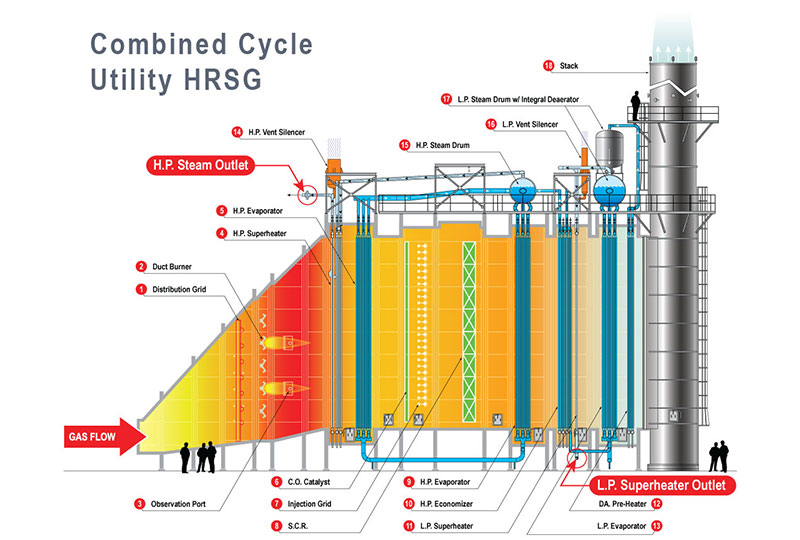
\includegraphics[width=0.8\textwidth]{image.png}
  \caption{System Overview}
  \label{fig:image1}
\end{figure}

\section{Energy Calculations}
\subsection{Heat Required for Water}
The energy required to heat 180,000 liters of water per day by 40°C is calculated as:
\[
Q_{\text{water}} = \text{Volume} \times \text{Density} \times C_{p_{\text{water}}} \times \Delta T = 180,000 \, \text{liters} \times 1 \, \text{kg/liter} \times 4.186 \, \text{kJ/kg}^\circ\text{C} \times 40^\circ\text{C}
\]
\[
Q_{\text{water}} = 30139200 \, \text{kJ/day}
\]
Converted to average power:
\[
Q_{\text{water}} = \frac{30139200 \, \text{kJ}}{86400 \, \text{s}} \approx 348.83 \, \text{kW}
\]

\subsection{Input Energy for Gas Turbine}
The input energy required for the gas turbine is calculated by considering the efficiencies of the cycle, mechanical transmission, and the electrical generator. These efficiency values are based on typical performance data for contemporary gas turbine systems used in similar applications:
\begin{itemize}
    \item \textbf{Cycle Efficiency (0.35)}: This is the thermal efficiency of the gas turbine cycle, typically ranging from 33\% to 40\% for modern gas turbines under similar operational conditions. This specific value is chosen based on averages obtained from manufacturer data and industry benchmarks for gas turbines without heat recovery.
    \item \textbf{Mechanical Efficiency (0.98)}: This efficiency accounts for losses primarily due to mechanical friction and auxiliary systems that support the turbine operation. It is generally very high, reflecting the advanced design of turbines to minimize mechanical losses.
    \item \textbf{Generator Efficiency (0.95)}: Represents the efficiency of converting mechanical energy into electrical energy. Modern generators achieve efficiencies close to 95\%, with some variation based on load and operational conditions.
\end{itemize}

Given these efficiencies, the formula for the required input energy to meet the total power demand of 1116 kW is:
\[
\dot{W}_{\text{input}} = \frac{1116 \, \text{kW}}{0.35 \times 0.98 \times 0.95} \approx 3424.89 \, \text{kW}
\]

\subsection{Calculation of Recoverable Heat}
Given the high thermal output of the gas turbine and the efficiency of the HRSG, the calculations below summarize the available thermal energy and its potential uses:
\begin{itemize}
    \item Total energy input to the turbine: \(3424.89 \, \text{kW}\)
    \item Cycle efficiency of the turbine: \(35\%\)
    \item Thermal energy output (waste heat): \(3424.89 \, \text{kW} \times (1 - 0.35) = 2226.18 \, \text{kW}\)
    \item Efficiency of heat recovery (HRSG efficiency): \(80\%\)
    \item Recoverable heat: \(2226.18 \, \text{kW} \times 0.80 = 1780.94 \, \text{kW}\)
\end{itemize}

\subsection{Application of Recoverable Heat}
The recoverable heat of approximately \(1780.94 \, \text{kW}\) exceeds the required \(348.83 \, \text{kW}\) for heating 180,000 liters of water per day by \(40^\circ\text{C}\). This surplus allows not only for the complete supply of the hotel's hot water needs but also provides potential for additional applications:
\begin{itemize}
    \item \textbf{Heating Applications}: The excess heat can be utilized for heating swimming pools, spa facilities, or through radiators for space heating during cooler months.
    \item \textbf{Future Expansion}: As the hotel expands or if new facilities are added, this excess heat can be channeled to meet the increased demand, ensuring that the energy utilization remains highly efficient.
\end{itemize}

\section{Calculation of Daily Fuel Consumption}
To determine the daily fuel consumption of the gas turbine, several key parameters must be accurately assessed, including the total power requirement, the efficiency of the turbine, and the physical properties of natural gas.

\subsection{Given Data and Assumptions}
\begin{itemize}
    \item Total power requirement: \(1116 \, \text{kW}\)
    \item Efficiency of the power plant: \(35\%\)
    \item Heating value of natural gas: \(10.55 \, \text{kWh/m}^3\)
    \item Updated density of natural gas: \(2.83 \, \text{kg/m}^3\)
\end{itemize}

\subsection{Fuel Consumption Calculation}
The volume of natural gas required per day is determined based on the energy output needed and the efficiency of the turbine. The formula used is:
\[ \text{Volume of Gas per Day} = \frac{\text{Total Power Requirement} \times 24}{\text{Efficiency} \times \text{Heating Value}} \]
\[ \text{Volume of Gas per Day} = \frac{1116 \, \text{kW} \times 24}{0.35 \times 10.55 \, \text{kWh/m}^3} \approx 7253.62 \, \text{m}^3/\text{day} \]

The mass of natural gas needed per day is then calculated by multiplying the volume by the updated density:
\[ \text{Mass of Gas per Day} = \text{Volume of Gas per Day} \times \text{Density of Natural Gas} \]
\[ \text{Mass of Gas per Day} = 7253.62 \, \text{m}^3/\text{day} \times 2.83 \, \text{kg/m}^3 \approx 20527.75 \, \text{kg} \]

\section{Fuel Cost Calculation}
This section updates the previous fuel cost calculations for a gas turbine power plant, utilizing the latest natural gas price of \$4.96 per 1,000 cubic feet. The new calculations adjust the cost per cubic meter and reevaluate the daily fuel cost and cost per kWh.

\subsection{Conversion of Natural Gas Price}
\begin{itemize}
    \item Original price: \$4.96 per 1,000 cubic feet
    \item Converted price per cubic meter: \$0.1752
\end{itemize}

\subsection{Updated Calculation of Total Daily Fuel Cost}
The total daily fuel cost, based on the required volume of natural gas (7253.62 m³/day), is recalculated with the updated price:
\[ \text{Total Daily Fuel Cost} = 7253.62 \, \text{m}^3/\text{day} \times \$0.1752/\text{m}^3 = \$1270.55 \]

\subsection{Updated Calculation of Cost per kWh}
The cost per kWh is updated based on the new total daily fuel cost:
\[ \text{Cost per kWh} = \frac{\$1270.55}{1116 \, \text{kW} \times 24 \, \text{hours}} \approx \$0.0474/\text{kWh} \]


\section*{Equations}
\begin{equation}
Q_{\text{air, in}} = \dot{m}_{\text{dry air}} \times C_{p_{\text{air}}} (\Delta T)
\end{equation}
\begin{equation}
\dot{V}_{\text{moist air}} = \dot{V}_{\text{air total}} \times \text{humidity ratio}
\end{equation}
\begin{equation}
\dot{V}_{\text{dry air}} = \dot{V}_{\text{air total}} - \dot{V}_{\text{moist air}}
\end{equation}
\begin{equation}
\dot{m}_{\text{dry air}} = \frac{P\dot{V}_{\text{dry air}}}{\bar{R}T/M}
\end{equation}
\begin{multline}
Q_{\text{tot}} = Q_{\text{air, in}} + 5.0 \left(\frac{\text{KW}}{K}\right)(T_{\text{inside}} - T_{\text{outside}}) - 0.45(\text{Building Electric Demand}) - 12 \text{ kW}
\end{multline}
\begin{equation}
Q_{\text{water}} = \dot{m}_{\text{water}} \times C_{p_{\text{water}}} (T_H - T_C)
\end{equation}
\begin{equation}
\dot{W}_{\text{cycle}} = \frac{Q_{\text{air in}}}{h_1 - h_4} (h_2 - h_1)
\end{equation}
\begin{equation}
\dot{W}_{\text{compressor}} = \dot{m}_{\text{air}} (h_{2s} - h_1)
\end{equation}

\section*{References}
Fundamentals of Engineering Thermodynamics, 8th Ed.

Wikipedia (\url{https://en.wikipedia.org/wiki/Heat_recovery_steam_generator} [Accessed: 25-April-2024]).

\end{document}